\documentclass[spanish,a4paper,14pt,oneside]{extreport}

%%%%%%%%%%%%%%%%%%%%%%%%%%%%%%%%%%%%%%%%%%%%%%%%%%%%%%%%%%%%%%%%%%%%%%%%%%%%%%%
\usepackage[dvips]{graphicx}
\usepackage[dvips]{epsfig}
\usepackage[utf8]{inputenc}
\usepackage[spanish]{babel}
\usepackage{alltt}
\usepackage{algorithm}
\usepackage{algorithmic}
\usepackage{multirow}
\usepackage{hyperref}
\usepackage{color}
\usepackage[top=2cm, bottom=2cm, left=2cm, right=2cm]{geometry}

%%%%%%%%%%%%%%%%%%%%%%%%%%%%%%%%%%%%%%%%%%%%%%%%%%%%%%%%%%%%%%%%%%%%%%%%%%%%%%%

\newcommand{\SONY}{{\sc Sony}}
\newcommand{\MICROSOFT}{{\sc Microsoft}}
\newcommand{\GCC}{\textsf{\textsc{G}CC}}
\newcommand{\INTEL}{\textsf{\textsc{I}ntel}}

%%% Traducimos el pseudocodigo
\renewcommand{\algorithmicwhile}{\textbf{mientras}}
\renewcommand{\algorithmicend}{\textbf{fin}}
\renewcommand{\algorithmicdo}{\textbf{hacer}}
\renewcommand{\algorithmicif}{\textbf{si}}
\renewcommand{\algorithmicthen}{\textbf{entonces}}
\renewcommand{\algorithmicrepeat}{\textbf{repetir}}
\renewcommand{\algorithmicuntil}{\textbf{hasta que}}
\renewcommand{\algorithmicelse}{\textbf{en otro caso}}
\renewcommand{\algorithmicfor}{\textbf{para}}

%\newcommand{\RETURN}{\textbf{retornar} }
\newcommand{\RET}{\STATE \textbf{retornar} }
\newcommand{\TO}{\textbf{hasta} }
\newcommand{\AND}{\textbf{y} }
\newcommand{\OR}{\textbf{o} }

%%%%%%%%%%%%%%%%% Creamos un entorno para listar código fuente %%%%%%%%%%%%%%%
\newenvironment{sourcecode}
{\begin{list}{}{\setlength{\leftmargin}{1em}}\item\scriptsize\bfseries}
{\end{list}}

\newenvironment{littlesourcecode}
{\begin{list}{}{\setlength{\leftmargin}{1em}}\item\tiny\bfseries}
{\end{list}}

\newenvironment{summary}
{\par\noindent\begin{center}\textbf{Abstract}\end{center}\begin{itshape}\par\noindent}
{\end{itshape}}

\newenvironment{keywords}
{\begin{list}{}{\setlength{\leftmargin}{1em}}\item[\hskip\labelsep \bfseries Keywords:]}
{\end{list}}

\newenvironment{palabrasClave}
{\begin{list}{}{\setlength{\leftmargin}{1em}}\item[\hskip\labelsep \bfseries Palabras clave:]}
{\end{list}}


%%%%%%%%%%%%%%%%%%%%%%%%%%%%%%%%%%%%%%%%%%%%%%%%%%%%%%%%%%%%%%%%%%%%%%%%%%%%%%%
% Format
%%%%%%%%%%%%%%%%%%%%%%%%%%%%%%%%%%%%%%%%%%%%%%%%%%%%%%%%%%%%%%%%%%%%%%%%%%%%%%%
%\usepackage{showframe}
%\marginparwidth 0mm
%%\topmargin -4 mm
%\topmargin -21 mm
%\headheight 10 mm
%\headsep 10 mm

%\textheight 229 mm
%\textheight 246 mm

%\oddsidemargin -5.4 mm
%\evensidemargin -5.4 mm
%\oddsidemargin 5 mm
%\evensidemargin 5 mm

%\oddsidemargin -3 mm
%\evensidemargin -3 mm

%\textwidth 17 cm
%\textwidth 15 cm
%\columnsep 10 mm

\input{amssym.def}

%%%%%%%%%%%%%%%%%%%%%%%%%%%%%%%%%%%%%%%%%%%%%%%%%%%%%%%%%%%%%%%%%%%%%%%%%%%%%%%

\begin{document}

%%%%%%%%%%%%%%%%%%%%%%%%%%%%%%%%%%%%%%%%%%%%%%%%%%%%%%%%%%%%%%%%%%%%%%%%%%%%%%%
% First Page
%%%%%%%%%%%%%%%%%%%%%%%%%%%%%%%%%%%%%%%%%%%%%%%%%%%%%%%%%%%%%%%%%%%%%%%%%%%%%%%

\pagestyle{empty}
\thispagestyle{empty}


\newcommand{\HRule}{\rule{\linewidth}{1mm}}
\setlength{\parindent}{0mm}
\setlength{\parskip}{2.5mm}

\vspace*{\stretch{0.5}}

\begin{center}

\includegraphics[scale=0.8]{images/logo_vertical}\\[10mm]
{\Huge Trabajo de Fin de Grado}
\end{center}

\HRule
\begin{flushright}
        {\Huge CodeLab} \\[2.5mm]
        {\Large A Tool to automate repository creation and access control, giving support to distribute starter code, collect assignments and evaluate the students work on GitHub.} \\[5mm]
        {\Large Samuel Ramos Barroso} \\[5mm]


\end{flushright}
\HRule
\vspace*{\stretch{2}}
\begin{center}
  \Large La Laguna, \today
\end{center}

\setlength{\parindent}{5mm}

%%%%%%%%%%%%%%%%%%%%%%%%%%%%%%%%%%%%%%%%%%%%%%%%%%%%%%%%%%%%%%%%%%%%%%%%%%%%%%%
% Signature page (add the official stamp)
%%%%%%%%%%%%%%%%%%%%%%%%%%%%%%%%%%%%%%%%%%%%%%%%%%%%%%%%%%%%%%%%%%%%%%%%%%%%%%%
\newpage
%\cleardoublepage
\thispagestyle{empty}

D. {\bf Casiano Rodríguez León}, con N.I.F. 42.020.072-S profesor Catedratico de Universidad adscrito al Departamento de Lenguajes y Sistemas Informáticos de la Universidad de La Laguna, como tutor

\bigskip
\bigskip
{\bf C E R T I F I C A}

\bigskip
\bigskip
\bigskip
Que la presente memoria titulada:

\bigskip
``{\it CodeLab.}''

\bigskip
\bigskip
\bigskip

\noindent ha sido realizada bajo su dirección por D. {\bf Samuel Ramos Barroso},
con N.I.F. 51.165-611-H.

\bigskip
\bigskip

Y para que así conste, en cumplimiento de la legislación vigente y a los efectos oportunos firman la presente en La Laguna a \today

%\cleardoublepage
\newpage
%%%%%%%%%%%%%%%%%%%%%%%%%%%%%%%%%%%%%%%%%%%%%%%%%%%%%%%%%%%%%%%%%%%%%%%%%%%%%%%
\thispagestyle{empty}

{ \flushright

\begin{LARGE}
Agradecimientos
\end{LARGE}

\hspace{3mm}

\begin{large}

\hspace{3mm}
A mi familia, por el apoyo que me han dado durante estos años.

\hspace{3mm}
A Casiano, por enseñarme el mundo de las tecnologías web y transmitirme sus conocimientos sobre JavaScript e iniciarme en el mundo fullstack.

\end{large}

}

%%%%%%%%%%%%%%%%%%%%%%%%%%%%%%%%%%%%%%%%%%%%%%%%%%%%%%%%%%%%%%%%%%%%%%%%%%%%%%%%%
\newpage

\begin{huge}
Licencia
\end{huge}

\begin{center}

\includegraphics[scale=1.5]{images/by-nc_88x31}\\[10mm]
{\Large \copyright~Esta obra está bajo una licencia de Creative Commons Reconocimiento-NoComercial 4.0 Internacional.
}
\end{center}

%%%%%%%%%%%%%%%%%%%%%%%%%%%%%%%%%%%%%%%%%%%%%%%%%%%%%%%%%%%%%%%%%%%%%%%%%%%%%%%
\newpage  %\cleardoublepage
\begin{abstract}
{\em

Este proyecto trata sobre la creación plataforma web destinada al apoyo del profesorado para la realización de prácticas 
intentando resolver las limitaciones que tienen otras plataformas para la gestión de prácticas. 
El profesor podrá crear tareas que serán asignadas a sus alumnos de forma individual o grupal. 
Cada alumno realizará su trabajo en un repositorio git, el cual una vez finalizado, podrá ser revisado por el profesor.

}

\begin{palabrasClave}
Git, Github, Tareas, Clases, Prácticas de Programación.
\end{palabrasClave}

\end{abstract}
%%%%%%%%%%%%%%%%%%%%%%%%%%%%%%%%%%%%%%%%%%%%%%%%%%%%%%%%%%%%%%%%%%%%%%%%%%%%%%%

%%%%%%%%%%%%%%%%%%%%%%%%%%%%%%%%%%%%%%%%%%%%%%%%%%%%%%%%%%%%%%%%%%%%%%%%%%%%%%%
\newpage  %\cleardoublepage
\begin{summary}
{\em

This project deals with the creation of a web platform designed to give support to teachers for the realization
of programming labs. 
It tries to solve the limitations of  other platforms with the same goal. 
The teachers can create tasks that will be assigned to their students individually or in
groups. Each student will perform their work in a git repository, which once it is completed, can be reviewed by the teacher.
}

\begin{keywords}
Git, Github, Tasks, Classes, Programming Labs.
\end{keywords}

\end{summary}
%%%%%%%%%%%%%%%%%%%%%%%%%%%%%%%%%%%%%%%%%%%%%%%%%%%%%%%%%%%%%%%%%%%%%%%%%%%%%%%

%%%%%%%%%%%%%%%%%%%%%%%%%%%%%%%%%%%%%%%%%%%%%%%%%%%%%%%%%%%%%%%%%%%%%%%%%%%%%%%
\newpage{\pagestyle{empty}}
\thispagestyle{empty}

%%%%%%%%%%%%%%%%%%%%%%%%%%%%%%%%%%%%%%%%%%%%%%%%%%%%%%%%%%%%%%%%%%%%%%%%%%%%%%%


\pagestyle{myheadings} %my head defined by markboth or markright
% No funciona bien \markboth sin "twoside" en \documentclass, pero al
% ponerlo se dan un montón de errores de underfull \vbox, con lo que no se
% ha puesto.
\markboth{Samuel Ramos Barroso}{CodeLab}

%%%%%%%%%%%%%%%%%%%%%%%%%%%%%%%%%%%%%%%%%%%%%%%%%%%%%%%%%%%%%%%%%%%%%%%%%%%%%%%
%Numeracion en romanos
\renewcommand{\thepage}{\roman{page}}
\setcounter{page}{1}

%%%%%%%%%%%%%%%%%%%%%%%%%%%%%%%%%%%%%%%%%%%%%%%%%%%%%%%%%%%%%%%%%%%%%%%%%%%%%%%

\tableofcontents

%%%%%%%%%%%%%%%%%%%%%%%%%%%%%%%%%%%%%%%%%%%%%%%%%%%%%%%%%%%%%%%%%%%%%%%%%%%%%%%
\newpage{\pagestyle{empty}}

\listoffigures

%%%%%%%%%%%%%%%%%%%%%%%%%%%%%%%%%%%%%%%%%%%%%%%%%%%%%%%%%%%%%%%%%%%%%%%%%%%%%%%
\newpage{\pagestyle{empty}}

\listoftables

%%%%%%%%%%%%%%%%%%%%%%%%%%%%%%%%%%%%%%%%%%%%%%%%%%%%%%%%%%%%%%%%%%%%%%%%%%%%%%%
\newpage{\pagestyle{empty}}

%%%%%%%%%%%%%%%%%%%%%%%%%%%%%%%%%%%%%%%%%%%%%%%%%%%%%%%%%%%%%%%%%%%%%%%%%%%%%%%
%Numeracion a partir del capitulo I
\renewcommand{\thepage}{\arabic{page}}
\setcounter{page}{1}


\chapter{Introducción}
\label{chapter:intro}

%%%%%%%%%%%%%%%%%%%%%%%%%%%%%%%%%%%%%%%%%%%%%%%%%%%%%%%%%%%%%%%%%%%%%%%%%%%%%
% Chapter 1: Introducción 
%%%%%%%%%%%%%%%%%%%%%%%%%%%%%%%%%%%%%%%%%%%%%%%%%%%%%%%%%%%%%%%%%%%%%%%%%%%%%%%

%---------------------------------------------------------------------------------
\section{Herramientas para el apoyo del profesorado de informática}
\label{1:sec:1}

En los últimos años se han desarrolladon las nuevas tecnologías, lo que ha permitido que lleguen nuevas herramientas de aprendizaje y de apoyo a la docencia. Es el caso de la exitosa plataforma Moodle, un LCMS, sigla de Learning Content Management System. 

El Moodle, como otros LCMS, se utiliza para crear y manejar el contenido de un programa educativo, como por ejemplo un curso. Normalmente se crean partes de contenido en forma de módulos que se pueden personalizar.

Existen otras herramientas como el LMS sigla de Learning Management System. El LMS es un software instalado en un servidor que se emplea para administrar, distribuir y controlar las actividades de formación de una institución. Un LCMS suele estár integrado en un LMS.

Las principales funciones del LMS son: gestionar usuarios, recursos, materiales y actividades de formación, administrar el acceso, controlar y hacer seguimiento del proceso de aprendizaje, realizar evaluaciones, generar informes, gestionar servicios de comunicación como foros de discusión, videoconferencias y correo electrónico entre otros.

Como ejemplos reales de las definiciones mencionadas, se encuentra el servicio LCMS de Google, Google Classroom que está basado en Moodle, con la diferencia de que usa la Suite de Google Drive para el apoyo de almacenamiento y gestión de tareas.

En el caso del apoyo al profesorado de informática encontramos los VPL sigla de Virtual Programing Lab, que es un módulo para la plataforma Moodle. Los VPL permiten editar y ejecutar el código fuente de las tareas de programación en el navegador, además permite que el profesor pueda corregir sin necesidad de descargar el código fuente para ejecutarlo, también se permite añadir restricciones como pegar código externo y permite comparar la similitud entre códigos de los alumnos, entre otras cosas.

Por último, la única herramienta para la gestión de tareas está desarrollada por Github, se trata de Github Classroom, una plataforma aprovecha las organizaciones y repositorios de Github como estructura para las aulas y tareas, haciendo uso de la herramienta de control de versiones Git. En el siguiente punto hablaremos en profundiad de Github Education y Classroom.


%---------------------------------------------------------------------------------
\section{Github Education}
\label{1:sec:2}

Github Education es una plataforma desarrollada por Github que contiene varias herramientas para apoyar a los profesores en la asignación de tareas de programación:

\begin{itemize}
  \item Classroom
  \item Classroom Desktop
  \item Teachers Pet  
  \item Education Comunity
  \item Student Pack
\end{itemize}

Classroom es una herramienta destinada a profesores para gestionar el uso educativo de GitHub. Simplifica la asignación de tareas, automatizando la creación de repositorios git usando las organizaciones de Github como aulas y los repositorios como asignaciones, es una herramienta útil y sencilla de usar, tanto para profesores como para alumnos, pero tiene ciertos defectos, por ejemplo, no se puede crear un repositorio de evaluación que contenga las tareas de todos los alumnos, para eso se debe usar Classroom Desktop, es decir, se requiere de otra herramienta para una única funcionalidad, tampoco se puede acceder a los enlaces de travis, si la práctica requiere su uso, por último, tiene un sistema para asociar información a cada alumno que es bastante complejo de usar, ya que requiere introducir a mano cada usuario y la información que se desea asociar.

Teachers Pet es un CLI destinado a la administración de Education vía terminal, pero dejaron de desarrollarla porque para realizar ciertas tareas requería demasiadas opciones y los comandos eran demasiado largos.

Education Comunity es un foro para el intercambio de información entre alumnos, profesores, investigadores y desarrolladores.

Student Pack es un paquete que ofrece Github a los alumnos para mejorar su experiencia haciendo uso de Github para el desarrrollo de tareas.





%%%%%%%%%%%%%%%%%%%%%%%%%%%%%%%%%%%%%%%%%%%%%%%%%%%%%%%%%%%%%%%%%%%%%%%%%%%%%%%

\chapter{Plan de trabajo}
\label{chapter:dos}

%%%%%%%%%%%%%%%%%%%%%%%%%%%%%%%%%%%%%%%%%%%%%%%%%%%%%%%%%%%%%%%%%%%%%%%%%%%%%%%
% Chapter 2: Título del capítulo 2
%%%%%%%%%%%%%%%%%%%%%%%%%%%%%%%%%%%%%%%%%%%%%%%%%%%%%%%%%%%%%%%%%%%%%%%%%%%%%%%

\section{Objetivos}
\label{2:sec:1}

Los objetivos a desarrollar en este trabajo se definen a continuación:

\begin{itemize}
  \item {\bf A1.} Analizar otras plataformas  web existentes para la gestión del código de las prácticas de informática y su metodología de trabajo.
  \item {\bf A2.} Estudiar el funcionamiento de otras plataformas  web existentes para la gestión del código de las prácticas de informática.
  \item {\bf A3.} Estudiar las tecnologías a usar y enfocar el diseño de la plataforma web.
  \item {\bf A4.} Estudiar las funcionalidades que se van a incluir en la plataforma web.
  \item {\bf A5.} Crear una aplicación web básica que permita al usuario iniciar sesión con su cuenta de Github.
  \item {\bf A6.} Continuar con el desarrollo de la aplicación incluyendo las funcionalidades que solucionen las dificultades de otras plataformas  web existentes para la gestión del código de las prácticas de informática.
  \item {\bf A7.} Diseñar y desarrollar los estilos de las vistas.
\end{itemize}



\newpage
\section{Plan de trabajo}
\label{2:sec:2}

%--------------------------------------------------------------------------
\begin{table}[!ht]
\begin{center}
\begin{tabular}{|p{25mm}|p{50mm}|} \hline 
\textbf{Objetivo} & \textbf{Fecha} \\ \hline

A1 &30 Enero - 3 Febrero \\
\hline

A2 & 4 - 9 Febrero 
\\
\hline

A3 & 10 - 15 Febrero 
\\
\hline

A4 & 
16 - 21 Febrero 
\\
\hline

A5 & 
22 Febrero - 22 Marzo 
\\
\hline

A6 & 
23 Marzo - 23 Mayo
\\
\hline

A7 &
25 Abril - 20 Junio
\\
\hline

\end{tabular}
\end{center}
\caption{Tabla resumen del plan de trabajo}
\label{table:resOthers}
\end{table}

%%%%%%%%%%%%%%%%%%%%%%%%%%%%%%%%%%%%%%%%%%%%%%%%%%%%%%%%%%%%%%%%%%%%%%%%%%%%%%%

\newpage{\pagestyle{empty}}
\thispagestyle{empty}

\chapter{Desarrollo del proyecto}
\label{chapter:tres}

%%%%%%%%%%%%%%%%%%%%%%%%%%%%%%%%%%%%%%%%%%%%%%%%%%%%%%%%%%%%%%%%%%%%%%%%%%%%%%%
% Chapter 3: Título del capítulo 3
%%%%%%%%%%%%%%%%%%%%%%%%%%%%%%%%%%%%%%%%%%%%%%%%%%%%%%%%%%%%%%%%%%%%%%%%%%%%%%%

\section{Tecnologías}
\label{3:sec1}

\subsection{Tecnologías populares}
\label{3:1:1}
{\bf Django - Python}
Django es un framework para aplicaciones web gratuito y open source, escrito en Python. Un conjunto de componentes que te ayudan a desarrollar sitios web más fácil y rápidamente siguiendo el patrón Modelo Vista Controlador.

{\bf Ruby on Rails - Ruby}
Ruby on Rails, también conocido como RoR o Rails, es un framework de aplicaciones web de código abierto escrito en el lenguaje de programación Ruby, siguiendo el patrón Modelo Vista Controlador (MVC).

{\bf Express.js - Javascript}
Espress.js  es un framework de desarrollo de aplicaciones web minimalista y flexible para Node.js. Está inspirado en Sinatra, además es robusto, rápido, flexible y muy simple, además, es compatible con el patrón Modelo Vista Controlador.

Aquí tenemos una pequeña comparación de la popularidad que han tenido estas tecnologías en el último año.

\subsection{Tecnologías Escogidas}
\label{3:1:2}

Finalmente se escogió Express.js, Node.js y Javascript como tecnologías principales a usar en este proyecto por las siguientes razones:

En primer lugar, el uso de Node.js como tecnología de servidor aporta una gran ventaja ya que Javascript se usa en ambos lados, en el backend y en el frontend, reduciendo complejidad y tiempo de desarrollo ya que Express es bastante fácil de aprender y usar. Además, JavaScript es el lenguaje de programación más popular en el desarrollo web.

\begin{figure}[!th]
\begin{center}
\includegraphics[scale=0.5]{images/comparativa}
\caption{Comparativa de Tecnologias usadas}
\label{fig:Comparativa de Tecnologias usadas}
\end{center}
\end{figure}

Además de eso, la comunidad de Node.js está en constante crecimiento: la cantidad de preguntas de StackOverflow aumenta constantemente, por lo que la base de conocimiento para la tecnología es amplia. También hay que destacar el hecho de que Node.js sea de código abierto y gratuito. 

Finalmente, Node nos ofrece NPM, un gestor de paquetes que dispone de una gran cantidad de paquetes que crece rápidamente y aporta una forma sencilla de gestionar los paquetes que necesitemos en nuestro proyecto.

{\bf NPM}

NPM es un administrador de paquetes para Node.js con cientos de miles de paquetes. Aunque crea parte de la estructura del directorio del proyecto, este no es el objetivo principal.

El objetivo principal, es la automatización de dependencias y gestión de paquetes de cada proyecto. Esto significa que puede especificar todas las dependencias de su proyecto dentro del fichero package.json usando el comando npm i -s nombrepaquete, de forma que cada vez que un usuario clone el proyecto en su máquina simplemente tenga ejecutar npm install e inmediatamente se descargan e instalan todas las dependencias necesarias para el funcionamiento del proyecto en el directorio node modules/. Además, también sirve para especificar en qué versión está su proyecto.

También es posible descargar manualmente los paquetes, copiarlo en el directorio nodemodules/ y usarlo de esa manera. Sin embargo, a medida que crezca el proyecto y la lista de dependencias, llevará mucho tiempo instalar los paquetes necesarios y será una tarea engorrosa. También hace que colaborar y compartir tu proyecto sea mucho más difícil

{\bf Express.js}

Express es un framework ‘’minimalista’’ que permite crear una infraestructura web simple sobre Node.js. Express permite crear una API REST, un tipo de arquitectura de desarrollo web que se apoya totalmente en el estándar HTTP:

\begin{itemize}
  \item GET: Para consultar y leer recursos
  \item POST: Para crear recursos
  \item PUT: Para editar recursos
  \item DELETE: Para eliminar recursos
  \item PATCH: Para editar partes concretas de un recurso
\end{itemize}

Express también permite crear una aplicación web siguiendo el patrón de diseño Modelo Vista Controlador, que separa los datos y la lógica de de una aplicación de su representación.

{\bf Github API}

Para poder usar Github como estructura necesitaremos hacer uso de su Github REST API v3. 
La API nos permitirá acceder a los servicios que ofrece Github de forma externa, es decir, podremos crear repositorios, usar organizaciones como clases y manejar otros servicios, como consulta de información sobre el usuario.
Para poder acceder a la clave de cada usuario, debemos usar un Token generado por Github, es decir, una cadena que nos permitirá  identificarnos para realizar transacciones usando la API, en este caso, el token será generado usando las aplicaciones OAuth que nos ofrece Github para que el usuario haga login con su cuenta de usuario de github, sin necesidad de poner su usuario y contraseña de Github en la plataforma Codelab.
La Github REST API v3 tiene además varias librerías de terceros y tres librerías oficiales escritas en Ruby, Javascript y .Net.

{\bf MongoDB}

MongoDB es un sistema gestor de base de datos NoSQL, es decir, MongoDB es un sistema de bases de datos no relacional, en lugar de almacenar los datos en tablas, se almacenan colecciones o documentos, que está formado por objetos, y estos a su vez por claves y cada clave tiene un valor asociado. Es decir, sería algo parecido a un documento JSON, aunque en MongoDB usan una distribución llamada BSON.

\begin{figure}[!th]
\begin{center}
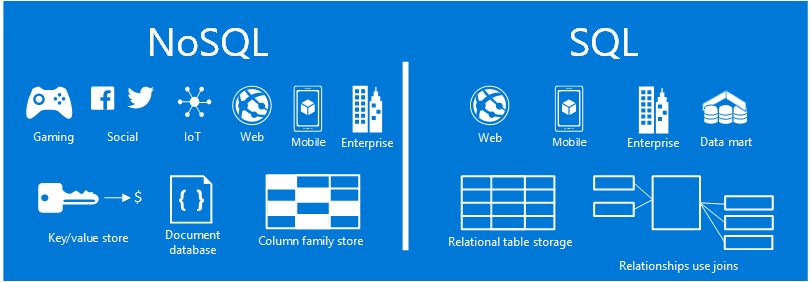
\includegraphics[scale=0.5]{images/nosql}
\caption{NoSQL vs SQL}
\label{fig:NoSQL vs SQL}
\end{center}
\end{figure}

{\bf Mongoose}

Mongoose es un una herramienta para el diseño de objetos de MongoDB. 
Mongoose provee una serie de métodos y funciones para manejar la base de datos en MongoDB.

{\bf Motor de vistas}

Como motor de vistas para el proyecto se ha elegido Pug, antes conocido como Jade, un motor de vistas implementado en Javascript para su uso en NodeJS y que dispone de una fácil integración con Express.JS. 

{\bf Automatización de tareas}

Para la automatización de tareas como generar el fichero de variables de entorno o poner en marcha un servidor nodemon se ha usado Gulp, una herramienta que permite automatizar tareas en Node.js, es simple y bastante fácil de usar.

{\bf Framework de CSS}

Como framework para los estilos de CSS se ha usado Materialize CSS, basado en material design. Ofrece varias opciones a la hora de diseñar la plataforma, permitiendo un diseño más minimalista o un diseño más cargado y vistoso.

%++++++++++++++++++++++++++++++++++++++++++++++++++++++++++++++++++++++++++++++
\section{Github API}
\label{3:sec2}

Para poder usar Github como estructura para la creación de aulas y tareas de código usaremos la Github REST API V3.
La API permite acceder a las funcionalidades de Github, A continuación se detallará que funcionalidades de la Github API se han usado

\begin{itemize}
  \item Oauth
  \item Organizaciones, Repositorios y Equipos
\end{itemize}

\subsection{OAuth}
\label{3:2:1}

La funcionalidad más básica que se usa es OAuth, que permite loguear al ususario con su cuenta de Github en
Codelab.

OAuth, sigla de Open Authorization es un estándar de código abierto que permite a un usuario compartir su información de un proveedor de servicios, como Google, Twitter, Facebook o en este caso de Github, con un consumidor, en nuestro caso Codelab.

Desde el punto de vista de Codelab, OAuth proporciona un método de acceso a los datos de Github a la vez que se protegen los credenciales de la cuenta.

Desde Codelab, solicitamos al usuario una serie de accesos y permisos en sus datos, para poder operar con las organizaciones y repositorios de Github.

\begin{figure}[!th]
\begin{center}
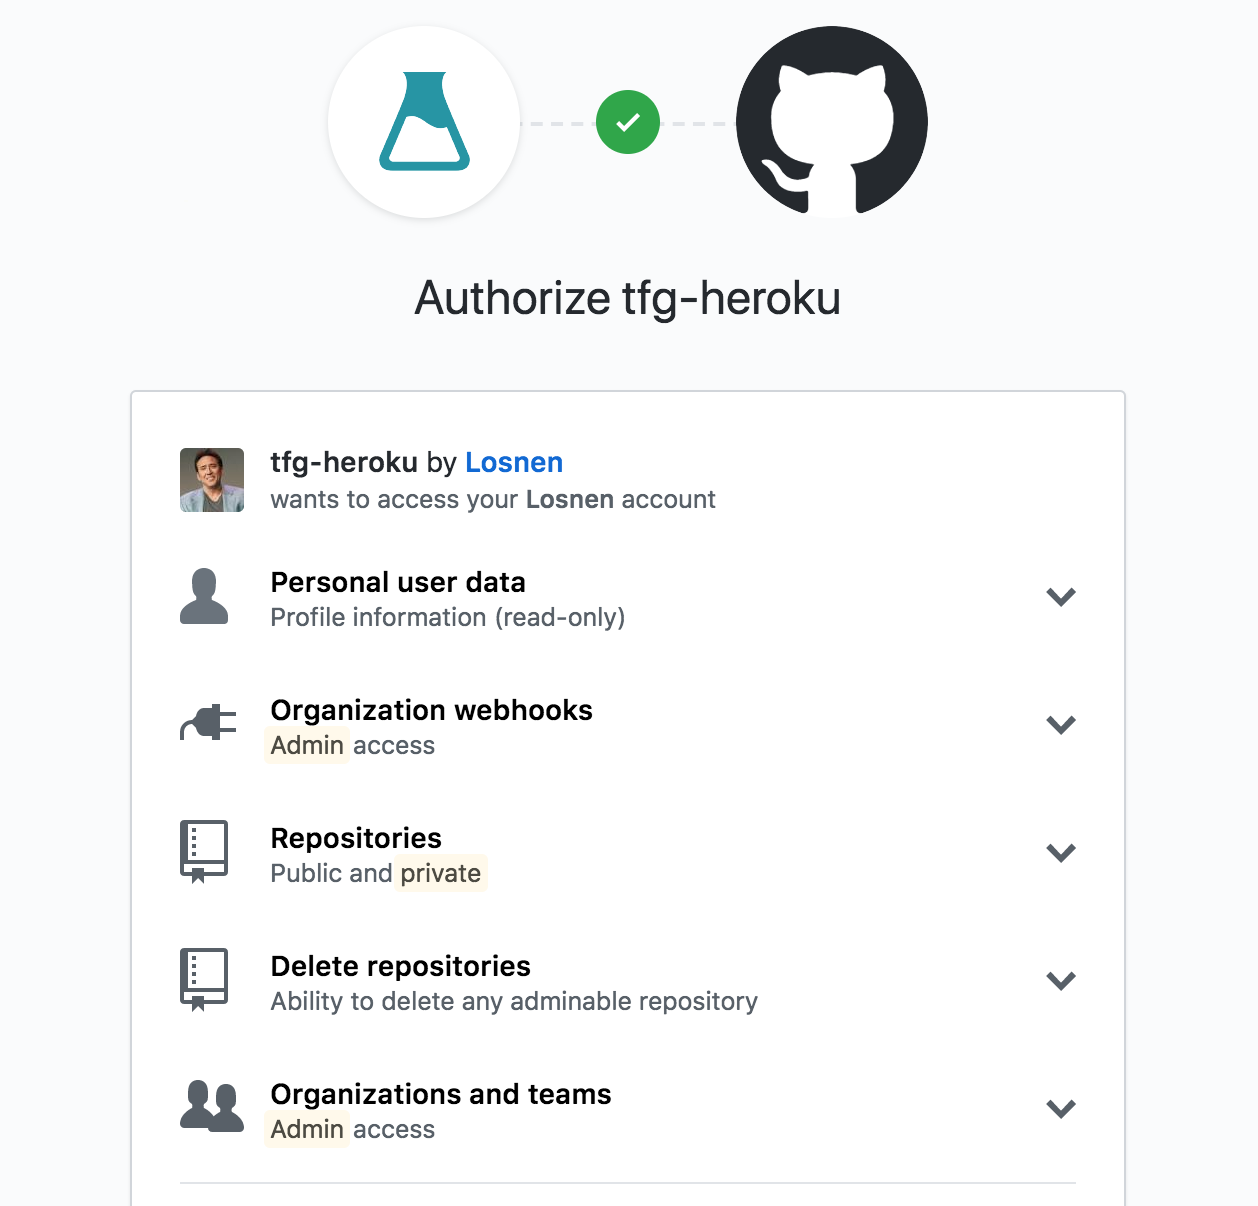
\includegraphics[scale=0.5]{images/permisos}
\caption{Vista de autorización de la OAuth App}
\label{fig:Vista de la OAuth App}
\end{center}
\end{figure}

Para tener acceso a OAuth primero debemos crear ua aplicación de OAuth en Github, simplemente tenemos que facilitarle a Github el nombre de nuestra aplicación, el dominio y un Callback URI, que es donde el servicio de Github redirigirá al usuario después de autorizar o denegar su aplicación,
Github devolverá un API Key y un Secret API Key para que lo introduzcamos en la plataforma. 

Para simplificar el uso de OAuth en la plataforma, se usa un framework llamado Passport.js diseñado para simplificar el Sign up y Log in para Express.js y que permite el uso de Github OAuth, 
Passport nos solicita las claves de la API, un callback url y los scopes o permisos que el usuario debe aprobar, para devolver los datos solicitados al usuario en forma de token para poder acceder a las demás funcionalidades de la Github API.

\subsection{Organizaciones, repositorios y equipos}
\label{3:2:2}

El acceso a las organizaciones, repositorios y equipos se realiza mediante una librería oficial de Github para Node.js
llamada Octokit, que permite casi todas las funcionalidades de la Github REST API, además ofrece varias formas de llamar a sus funciones, mediante 
el uso de async/await, promise y callback.

Para abordar la gestión, se utiliza una clase llamada Github en la que el constructor inicializa la API con el token del usuario y cada método accede a una funcionalidad de la API.

\begin{figure}[!th]
\begin{center}
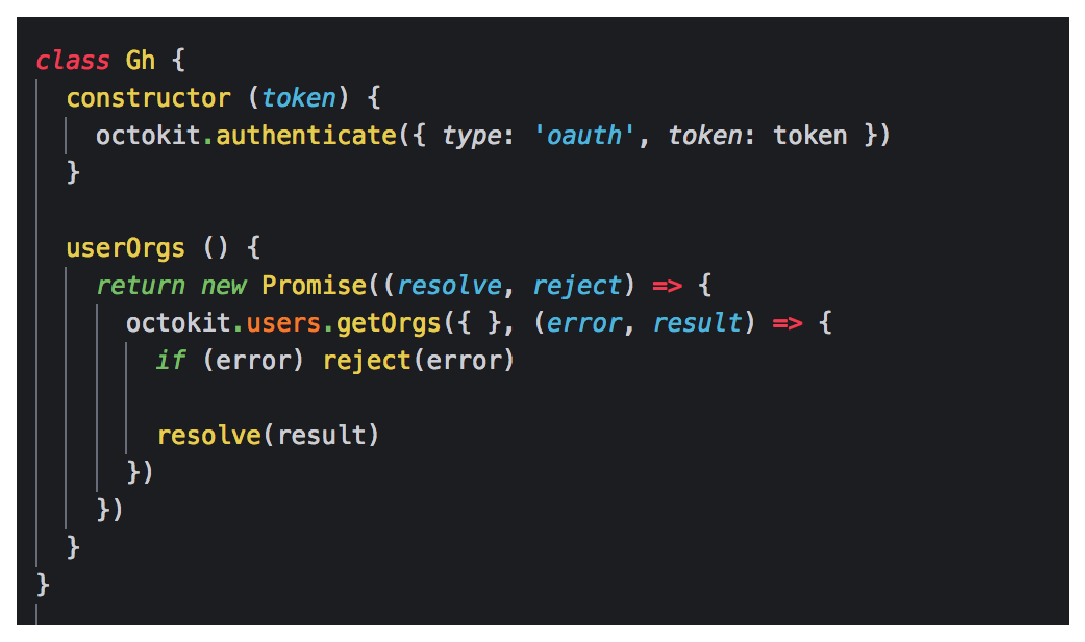
\includegraphics[scale=0.5]{images/clasegh}
\caption{Clase Github}
\label{fig:Clase Github}
\end{center}
\end{figure}

Las funcionalidades que aporta la API a Codelab son las siguientes:

\begin{itemize}
  \item Oauth
  \item Obtener las organizaciones del usuario para usar .
  \item Añadir usuarios a la organización.
  \item Crear un repositorio en las organizaciones.
  \item Añadir colaboradores al repositorio.
  \item Crear equipos.
  \item Añadir un equipo a un repositorio.
  \item Comprobar si un usuario es miembro de un equipo.
  \item Obtener los repositorios de una organización.
  \item Crear un fichero en un repositorio.
\end{itemize}

%++++++++++++++++++++++++++++++++++++++++++++++++++++++++++++++++++++++++++++++
\section{Modelo-Vista-Controlador}
\label{:sec3}

\subsection{El MVC}
\label{3:3:1}

El modelo vista controlador es una arquitectura de software que separa la lógica de la aplicación de la interfaz de usuario. Lo hace separando la aplicación en tres partes: el modelo, la vista y el controlador.

El modelo maneja los datos fundamentales, responde a las solicitudes de información, solicitudes para insertar, actualizar o eliminar la información. Esto podría ser una base de datos o cualquier sistema de estructura de datos. En resumen, es la gestión de datos y datos de la aplicación.

La vista proporciona la interfaz de usuario de la aplicación. Transformará los datos del modelo para mostrarselos al usuario de forma que pueda entender y manejar la información de forma sencilla e intuitiva.

El controlador recibe los datos y acciones del usuario y realiza llamadas al modelo para manejar los datos y a la vista para mostrar el resultado de dichas acciones.

\begin{figure}[!th]
\begin{center}
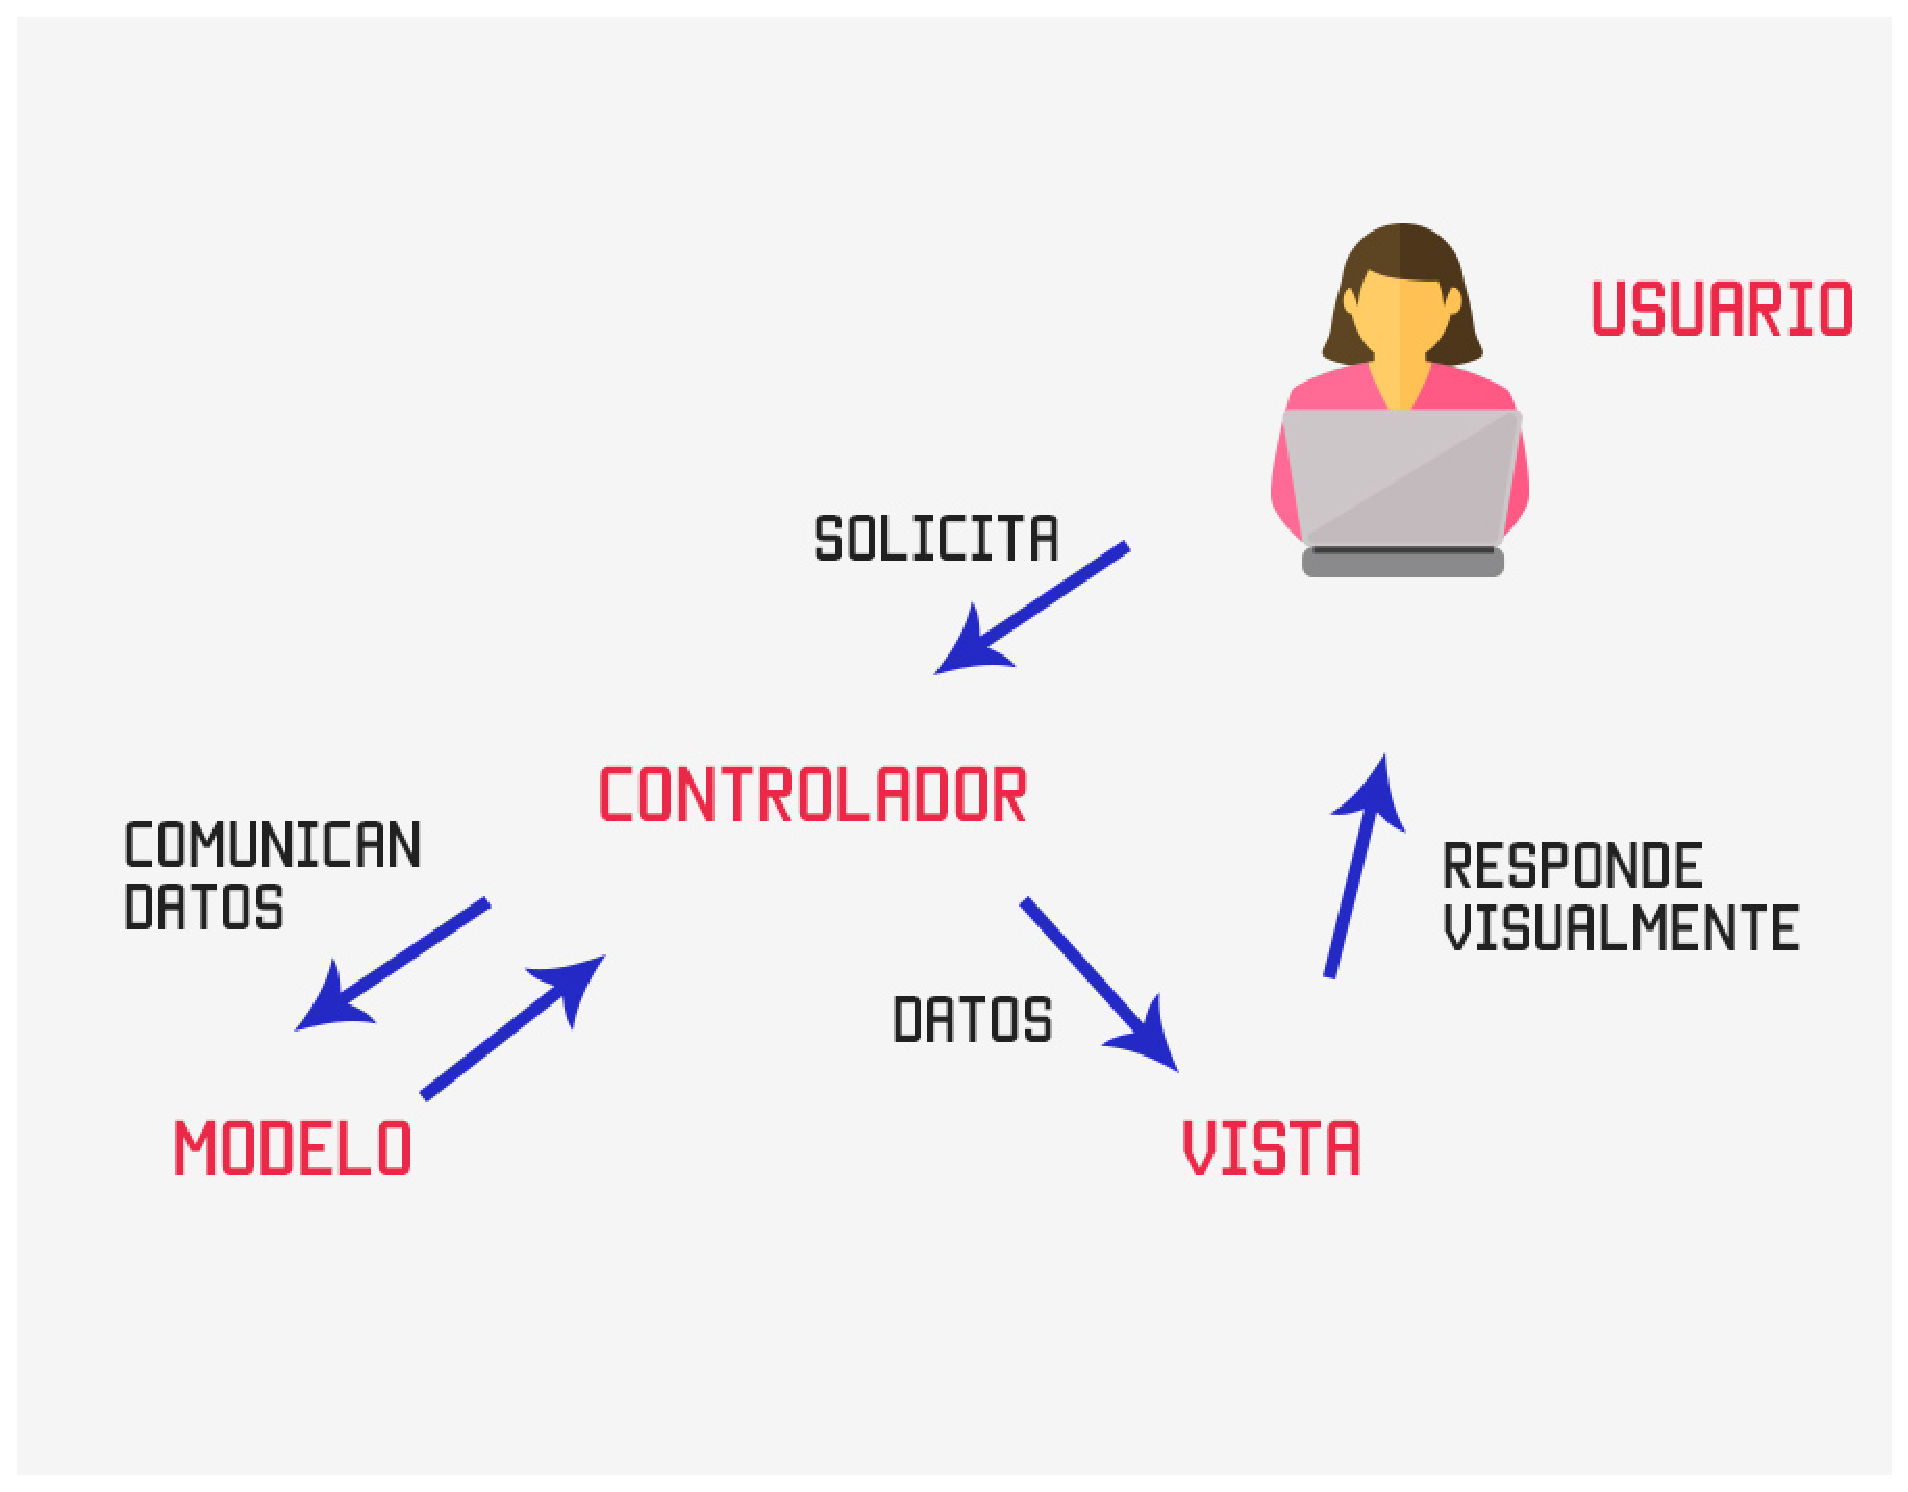
\includegraphics[scale=0.3]{images/29}
\caption{MVC}
\label{fig:MVC}
\end{center}
\end{figure}

\subsection{MVC en Codelab}
\label{3:3:2}

En la plataforma Codelab se ha implementado el Modelo Vista Controlador,
usando las funciones que nos proporciona Express.JS.

En el caso de las vistas Express nos permite establecer un motor de vistas.

\begin{figure}[!th]
\begin{center}
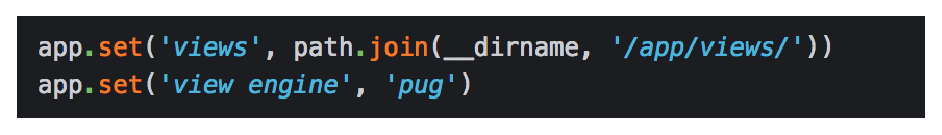
\includegraphics[scale=1.0]{images/defvistas}
\caption{Motor de vistas}
\label{fig:Motor de vistas}
\end{center}
\end{figure}

Con la primera línea de código le indicamos que la carpeta de vistas estará en el directorio app/views y con la segunda línea le indicamos que motor de vistas usaremos: Pug JS. 

En el código de abajo se puede ver la vista de error, que muestra al usuario el error y se le muestra el mensaje de error según el mensaje que se le pase desde el controlador.

\begin{figure}[!th]
\begin{center}
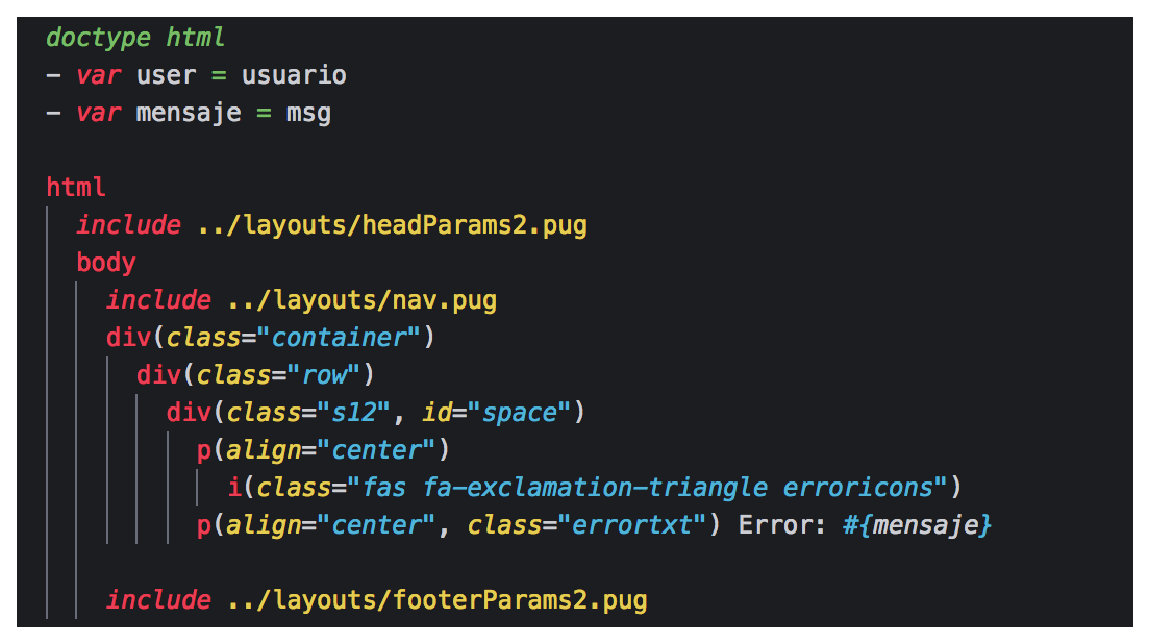
\includegraphics[scale=0.5]{images/vista}
\caption{Ejemplo de vista en Pug}
\label{fig:Ejemplo de vista en Pug}
\end{center}
\end{figure}

Pug es un motor de vistas bastante potente. Se pueden modular las vistas para reutilizar código y evitar repetirlo.
Por ejemplo, se puede dividir el código en Head donde se definen los distintos enlaces al CSS, JS y se pone el titulo, 
Nav que contiene la barra de navegación, que es igual para todos, el body que es el contenido de la vista y por último el footer.
También se pueden hacer bucles para mostrar las tareas o las aulas o mostrar un valor u otro dependiendo de si se tiene rol de alumno o de profesor.

\newpage

En el caso de los modelos se usa Mongoose y estarán ubicados en la carpeta de app/models. Los modelos le prorcionan la información a los controladores usando las funciones de mongoose, find, update, delete y save entre otras.

\begin{figure}[!th]
\begin{center}
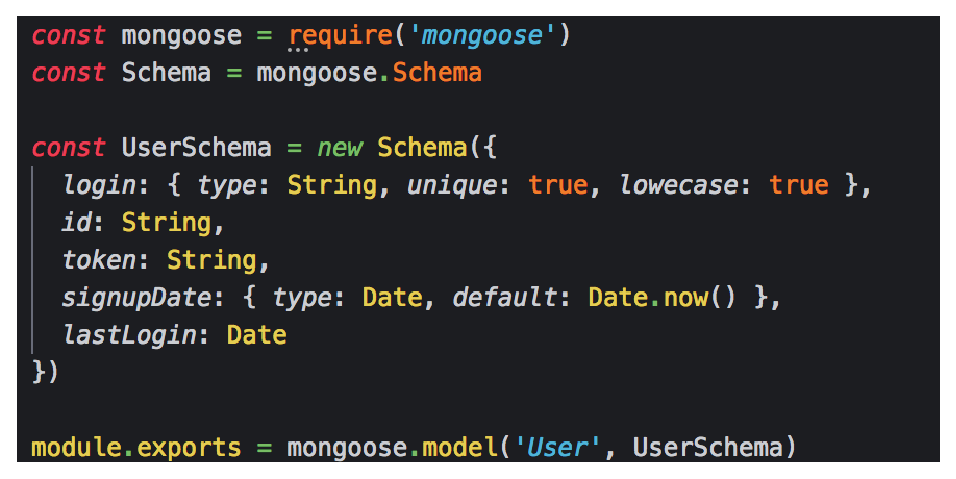
\includegraphics[scale=0.5]{images/modelo}
\caption{Ejemplo de modelo}
\label{fig:Ejemplo de modelo}
\end{center}
\end{figure}

Y por último, en el caso de los controladores, se definen funciones con las tareas que tienen que hacer
de forma que todo esta modulado. El controlador le pasa la información a las vistas usando el comando render, que renderiza la vista de Pug a HTML.


\begin{figure}[!th]
\begin{center}
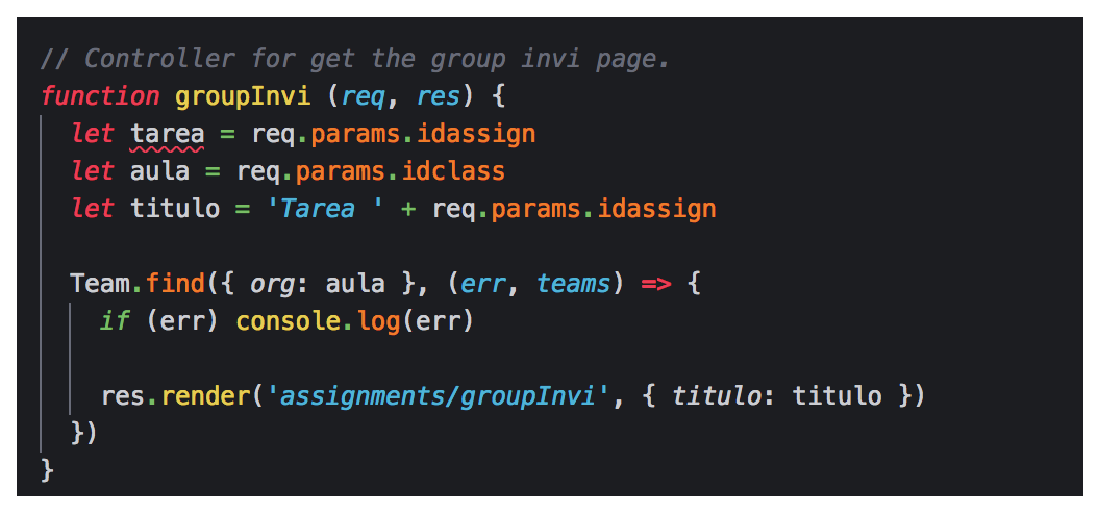
\includegraphics[scale=0.5]{images/controlador}
\caption{Ejemplo de Controlador}
\label{fig:Ejemplo de Controlador}
\end{center}
\end{figure}

Router se usa para crear rutas modulares. Una instancia Router es un sistema de middleware y direccionamiento completo que a menudo se denomina pequeña aplicación o miniapplicación.

Cabe destacar que para las rutas genéricas como aula o asignación en la que se puede representar los datos de cualquier aula o asignación se usan rutas que dependen de parámetos, es decir, rutas que muestran unos datos dependiendo de los parámetros que se le pasen.

\begin{figure}[!th]
\begin{center}
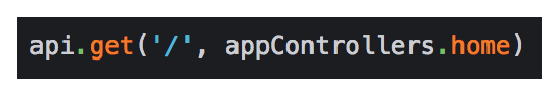
\includegraphics[scale=1.0]{images/ruta}
\caption{Ejemplo de ruta}
\label{fig:Ejemplo de ruta}
\end{center}
\end{figure}

%++++++++++++++++++++++++++++++++++++++++++++++++++++++++++++++++++++++++++++++

\section{Diseño de la base de datos}
\label{:sec4}

Se usará una base de datos NoSQL, en concreto MongoDB como sistema gestor y Mongoose como ODM, por lo que nos referimos las tablas como colecciones, columnas como claves y filas como objeto, todas las claves se escribirán usando el estilo camel case.

La base de datos es una parte muy importante de la plataforma, ya que en ella recae toda la responsabilidad de simular toda la estructura de aulas y tareas.

\subsection{Colección de usuarios}
\label{3:4:1}

Para almecenar los datos de los usuarios, existe una colección llamada user, donde se almacenarán datos como el id de github o el token:

\begin{itemize}
  \item login: Nombre de usuario de github, de tipo String y clave primaria.
  \item id: ID de github, de tipo string.
  \item token: Token para autorizar a la api de github, de tipo string.
  \item signupDate: Fecha en la que el usuario se registro, de tipo fecha
  \item lastLogin: Fecha en la que usuario se logueo por última vez, de tipo fecha.
\end{itemize}

\subsection{Colección de organizaciones}
\label{3:4:2}

Para almacenar los datos de las organizaciones existe una colección llamada orgs, que simula las aulas. Cada aula tendrá los siguientes datos:

\begin{itemize}
  \item login: Nombre de la organización en github, de tipo String y clave primaria.
  \item id: ID de github de la organización, de tipo string.
  \item avatar: Enlace a la foto de la organización, de tipo string.
  \item ownerID: ID del usuario dueño de la organización en github, de tipo string.
  \item ownerLogin: Nombre del usuario dueño de la organización en github, de tipo string.
  \item isActive: Booleano para identificar si las invitaciones a la organización están activas, de tipo boolean.
  \item createDate: Fecha en la que se registro la organización, de tipo fecha.
\end{itemize}

\subsection{Colección de asignaciones}
\label{3:4:3}

Para almacenar los datos de las tareas existe una colección llamada assigns, que simula las tareas. Cada tarea contendrá los siguientes datos:

\begin{itemize}
  \item title: Nombre de la tarea, de tipo String y clave primaria.
  \item ownerLogin: Nombre del usuario dueño de la tarea de tipo string.
  \item assignType: Tipo de aisngación, grupal o individual, de tipo string.
  \item repoType: Tipo de repositorio, privado o público, de tipo string.
  \item orgLogin: Nombre de la organización de github (aula) a la que pertenece la asignación, de tipo string.
  \item isActive: Booleano para identificar si las invitaciones a la tarea están activas, de tipo boolean.
  \item createDate: Fecha en la que se registro la tarea, de tipo fecha.
\end{itemize}

\subsection{Colección de asignaciones individuales}
\label{3:4:4}

Para almacenar los datos de las tareas individuales existe una colección llamada repos, que simula las tareas individuales. Cada tarea contendrá los siguientes datos:

\begin{itemize}
  \item name: Nombre del repositorio en github, de tipo String y clave primaria.
  \item assignName: Nombre de la tarea, de tipo string.
  \item StudentLogin: Nombre de github del alumno que realizará la tarea, de tipo string.
  \item ownerLogin: Nombre de github del dueño del aula, de tipo string
  \item orgLogin: Nombre de la organización de github (aula) a la que pertenece el repo, de tipo string.
  \item createDate: Fecha en la que se registro la tarea, de tipo fecha.
\end{itemize}

\subsection{Colección de asignaciones grupales}
\label{3:4:5}

Para almacenar los datos de las tareas grupales existe una colección llamada groups, que simula las tareas grupales. Cada tarea groupal contendrá los siguientes datos:

\begin{itemize}
  \item name: Nombre del repositorio en github, de tipo String y clave primaria.
  \item team: Nombre del equipo que realizará la tarea, de tipo string.
  \item idTeam: ID del equipo que realizará la tarea, de tipo string.
  \item assignName: Nombre de la tarea, de tipo string.
  \item StudentLogin: Nombre de github del alumno que realizará la tarea, de tipo string.
  \item ownerLogin: Nombre de github del dueño del aula, de tipo string
  \item orgLogin: Nombre de la organización de github (aula) a la que pertenece el repo, de tipo string.
  \item createDate: Fecha en la que se registro la tarea grupal, de tipo fecha.
\end{itemize}

\subsection{Colección de equipos}
\label{3:4:6}

Para almacenar los datos de los equipos existe una colección llamada teams. Cada equipo contendrá los siguientes datos:

\begin{itemize}
  \item name: Nombre del equipo, de tipo string.
  \item id: ID del equipo que realizará la tarea, de tipo string.
  \item members: Miembros que forman parte del equipo, de tipo array de string.
  \item orgLogin: Nombre de la organización de github (aula) a la que pertenece el equipo, de tipo string.
  \item createDate: Fecha en la que se registro el equipo, de tipo fecha.
\end{itemize}

\subsection{Colección de alumnos}
\label{3:4:7}

Para almacenar los alumnos de un aula existe una colección llamada students. Cada alumno tendrá los siguientes datos:

\begin{itemize}
  \item name: Nombre del alumno, de tipo string.
  \item surname: Apellido del alumno, de tipo string.
  \item email: Email del alumno, de tipo string.
  \item idGithub: Nombre de usuario del alumno en github, de tipo string
  \item createDate: Fecha en la que se registro el alumno de tipo fecha.
\end{itemize}
%++++++++++++++++++++++++++++++++++++++++++++++++++++++++++++++++++++++++++++++

\section{Descripción general de la plataforma web}
\label{:sec5}

Codelab es el nombre de la plataforma web que está destinada a simular el funcionamiento de un aula
que contiene tareas grupales o individuales sobre Github, es decir, como ya se ha mencionado anteriormente 
las organizaciones simularán las aulas y los repositorios las tareas.

\begin{figure}[!th]
\begin{center}

\includegraphics[scale=1.0]{images/probeta}
\end{center}
\end{figure}

\subsection{Diseño}
\label{3:5:1}

El diseño se realizó en Materialize CSS, un framework basando en material dessign. Como se puede apreciar, el diseño es bastante minimalista e intuitivo, aunque esté dirigido a un sector que maneja las nuevas tecgnoloías, se pretende que la plataforma sea lo más simple posible de manejar, tanto para profesores como para alumnos.
El usuario no debe registrarse, simplemente debe tener una cuenta de Github y loguearse con ella aceptando los permisos para poder ofrecerle los servicios de la plataforma, por lo que no es necesario rellenar ningun formulario de Log in o Sign Up.


\begin{figure}[!th]
\begin{center}
\includegraphics[scale=0.3]{images/landing}
\caption{Landing Page}
\label{fig:Landing page}
\end{center}
\end{figure}

\newpage

\subsection{Navegación}
\label{3:5:2}

La navegación dentro de la aplicación es bastante simple e intuitiva, existen dos barras de navegación:

La primera es la barra superior, que contiene los botones de Sign In si no se está logueado y los botones de Perfil, Aulas y Sign Out en caso de que se esté logueado.

\begin{figure}[!th]
\begin{center}
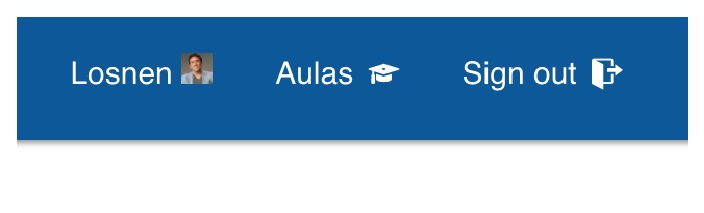
\includegraphics[scale=0.8]{images/nav}
\caption{Barra de navegación}
\label{fig:Barra de navegacion}
\end{center}
\end{figure}

La segunda está dentro de cada vista, si estamos en la vista de aulas veremos dos pestañas: Aulas y nueva Aula.

En cambio si estamos en la vista de aula veremos tareas, enlace de inivitación, nueva asignación, opciones, alumnos y subir fichero de alumnos.

Por último si nos encontramos en la vista de asignación se verá: repositorios, enlace de inivitación, repositorio de evaluación y opciones.

\begin{figure}[!th]
\begin{center}
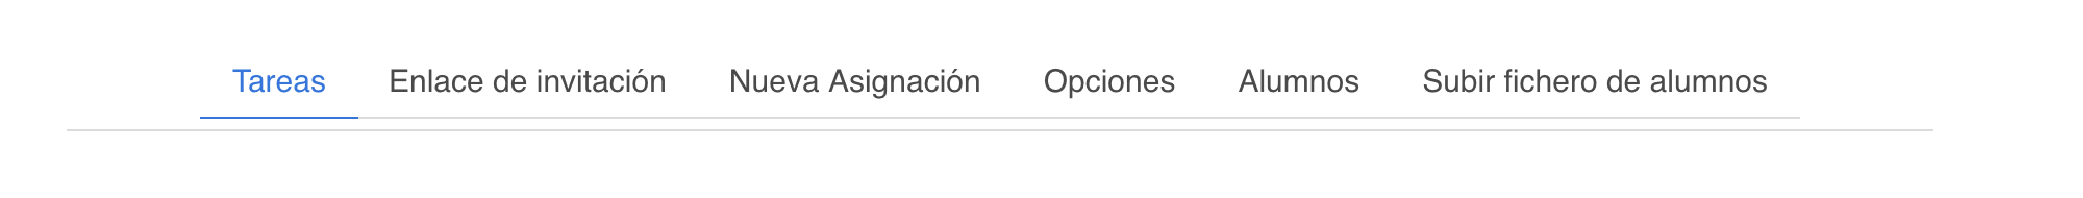
\includegraphics[scale=0.5]{images/navaula}
\caption{Barra de navegación de aula}
\label{fig:Barra de navegacion de aula}
\end{center}
\end{figure}
%++++++++++++++++++++++++++++++++++++++++++++++++++++++++++++++++++++++++++++++


\section{Funcionalidades}
\label{:sec6}

El proyecto se divide en tres paquetes de funcionalidades, Cada paquete incluye funcionalidades para cada rol:

\begin{itemize}
  \item Funcionalidades básicas
  \item Funcionalidades para profesores.
  \item Funcionalidades para el alumno
\end{itemize}

\subsection{Funcionalidades básicas}
\label{3:6:1}

Las funcionalidades básicas son comunes a todos los roles que participan en la plataforma, tanto alumnos como profesores, 

Todos los usuarios de la aplicación pueden hacer Log in, Log out y consultar un perfil.

En el perfil del usuario se puede consultar la información básica del usuario en Github, foto de perfil, nombre de usuario, correo y en el caso de que sea un alumno puede consultar las tareas que tiene en grupo o individualmente.

\begin{figure}[!th]
\begin{center}
\includegraphics[scale=0.2]{images/perfil}
\caption{Perfil de usuario}
\label{fig:Perfil de usuario}
\end{center}
\end{figure}

\newpage

\subsection{Funcionalidades para profesores}
\label{3:6:2}

Los profesores tendrán el grupo de funcionalidades más completo, ya que ellos son los protagonistas de la app, los profesores podrán desempeñar las siguientes tareas:

\begin{itemize}
  \item Añadir una organización como aula.
  \item Invitar alumnos al aula.
  \item Crear una tarea.
  \item Añadir un fichero de alumnos asociado al aula.
  \item Editar las opciones del aula.
  \item Invitar alumnos a la tarea.
  \item Editar las opciones de la tarea.
  \item Crear un repositorio de evaluación de cada tarea.
\end{itemize}

\subsubsection{Añadir una organización}

Añadir una organización como aula es la primera funcionalidad que puede desempeñar un profesor, en esta funcionalidad el profesor podrá elegir una organización de las que tenga creadas y a las que haya autorizado el acceso de terceros, 
es decir, el profesor tendrá que crear una organización y darle acceso de terceros antes de poder asignarla como aula en Codelab, una vez creado el aula, se le redirigirá al profesor a la vista donde puede ver todas sus aulas.

\begin{figure}[!th]
\begin{center}
\includegraphics[scale=0.4]{images/aula}
\caption{Aula}
\label{fig:Aula}
\end{center}
\end{figure}

\newpage
\subsubsection{Invitar alumnos al aula}

Para tenerlo todo bien organizado, será necesario tener a todos los alumnos incluidos de la organización de Github y que los alumnos tengan asignados el rol de miembro en lugar de colaboradores externos. Aunque las diferencias entre los colaboradores externos y los miembros son mínimas, 
es importante que los alumnos estén en la organización como miembros, ya que los colaboradores externos no tendrán acceso a todos los repositorios de la organización, sólo a aquellos en los que el profesor los incluya y además no podrán crear equipos, 
ver los miembros de la organización, ser un maintainer de un equipo o mencionar a otrose equipos visibles.

Por eso, el profesor podrá invitar a los alumnos a la organización mediante un enlace de invitación, que el alumno deberá aceptar para formar parte de la organización, así, el profesor podrá automatizar 
el proceso de admisión en el aula, sin tener que añadir alumnos uno a uno buscando por el identificador de Github.

Desde las opciones del aula el profesor podrá activar o desactivar las invitaciones para que sus alumnos puedan unirse.

\begin{figure}[!th]
\begin{center}
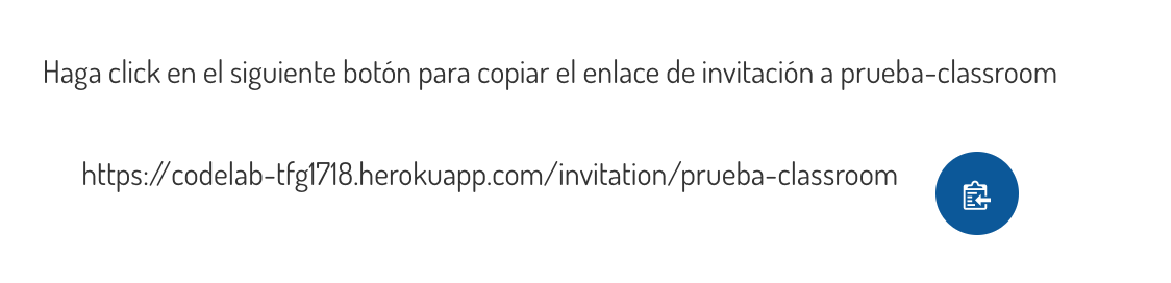
\includegraphics[scale=0.8]{images/invitacion}
\caption{Invitación}
\label{fig:Invitacion}
\end{center}
\end{figure}

\subsubsection{Crear una nueva tarea}

Esta funcionalidad destaca entre todas, crear la tarea es la funcionalidad más importante de la plataforma, ya que esta funcionalidad permite la automatización para la creación de los repositorios.
Si el profesor quiere crear una tarea es tan fácil como asignarle un título, elegir si el repositorio es público o privado y por último definir si la tarea es individual o grupal.

Después de crear la tarea, se redirigirá a la vista de la tarea, donde el profesor podrá gestionar las tareas de cada alumno. se podrá ver una breve información del usuario si el profesor añadió un fichero xslx o csv con la información de los alumnos.

En esa vista aparecerá un pequeño menú que tiene la pestaña descrita en el párrafo anterior, una pestaña para el enlace de invitación, una pestaña para crear el repositorio de evaluación una última pestaña de opciones, todas estas, son las opciones disponibles para operar con las tareas.

Desde las opciones de la tarea el profesor podrá activar o desactivar las invitaciones para que sus alumnos puedan unirse.

\begin{figure}[!th]
\begin{center}
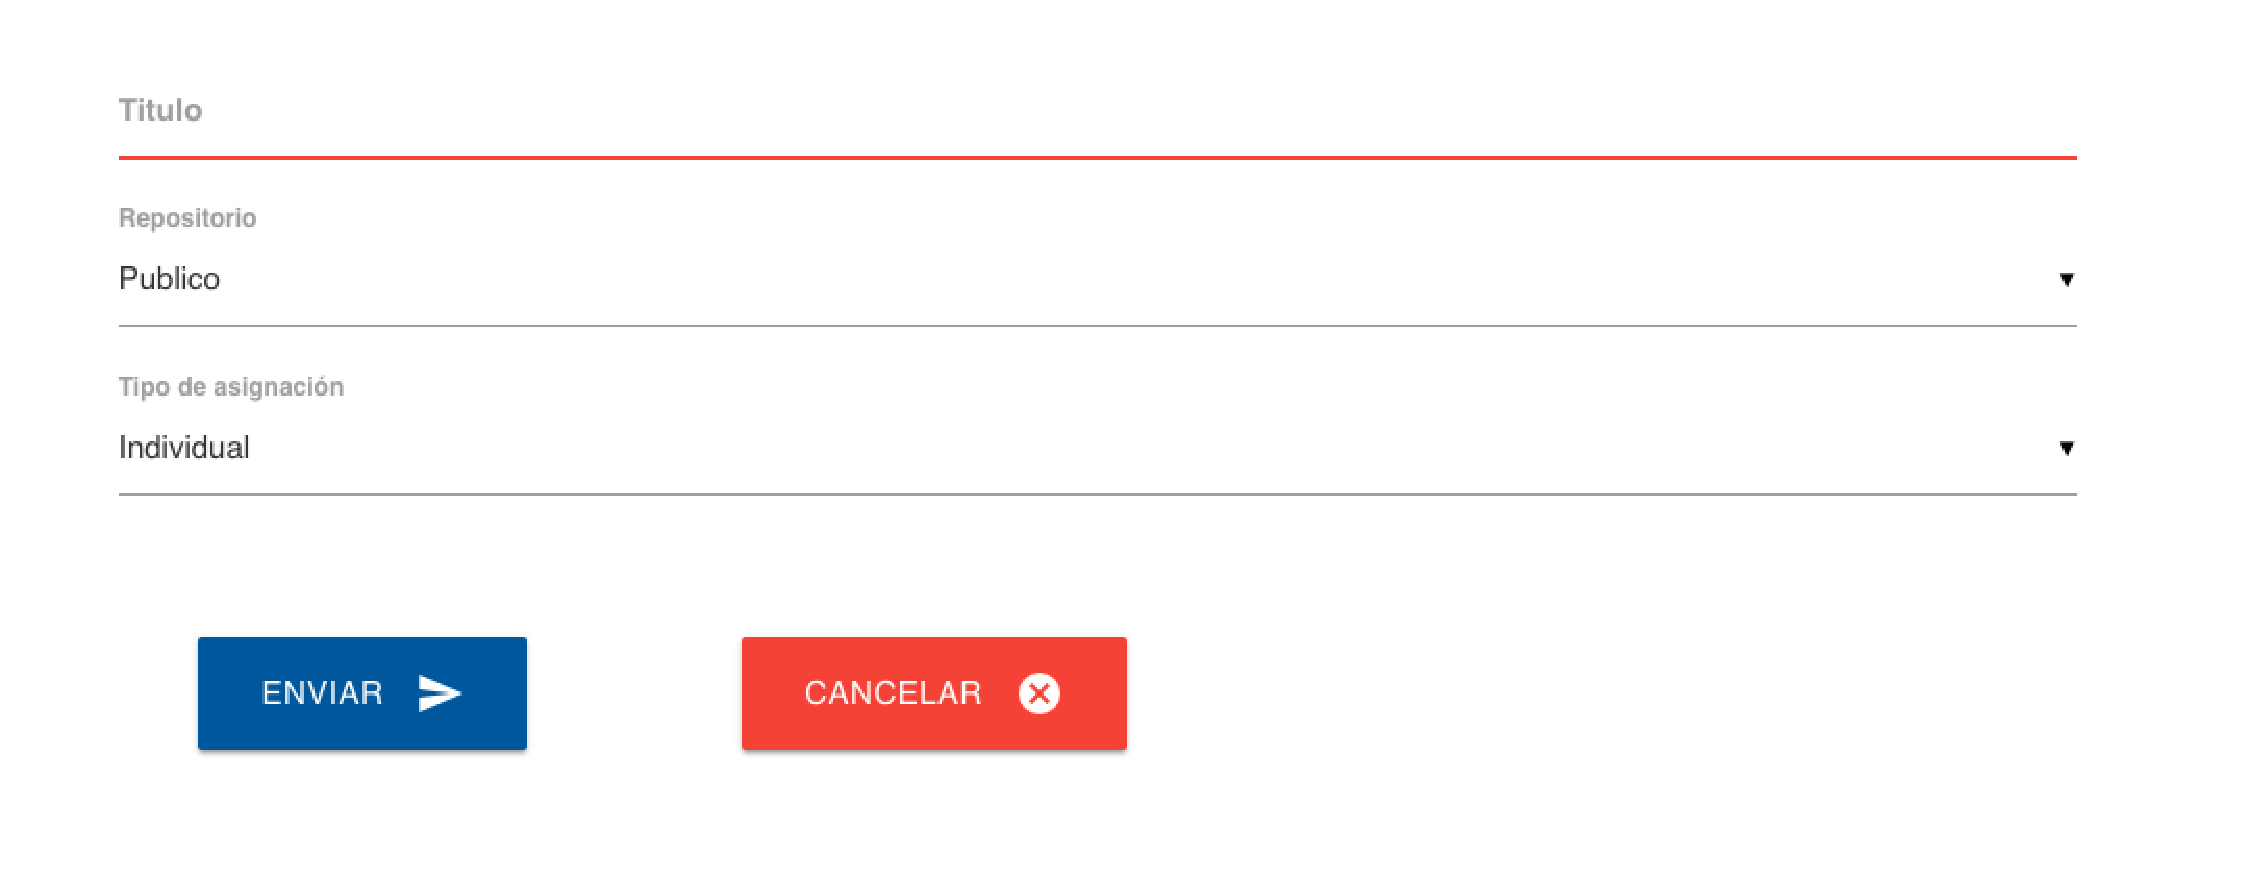
\includegraphics[scale=0.5]{images/tarea}
\caption{Nueva tarea}
\label{fig:Nueva tarea}
\end{center}
\end{figure}

\begin{figure}[!th]
\begin{center}
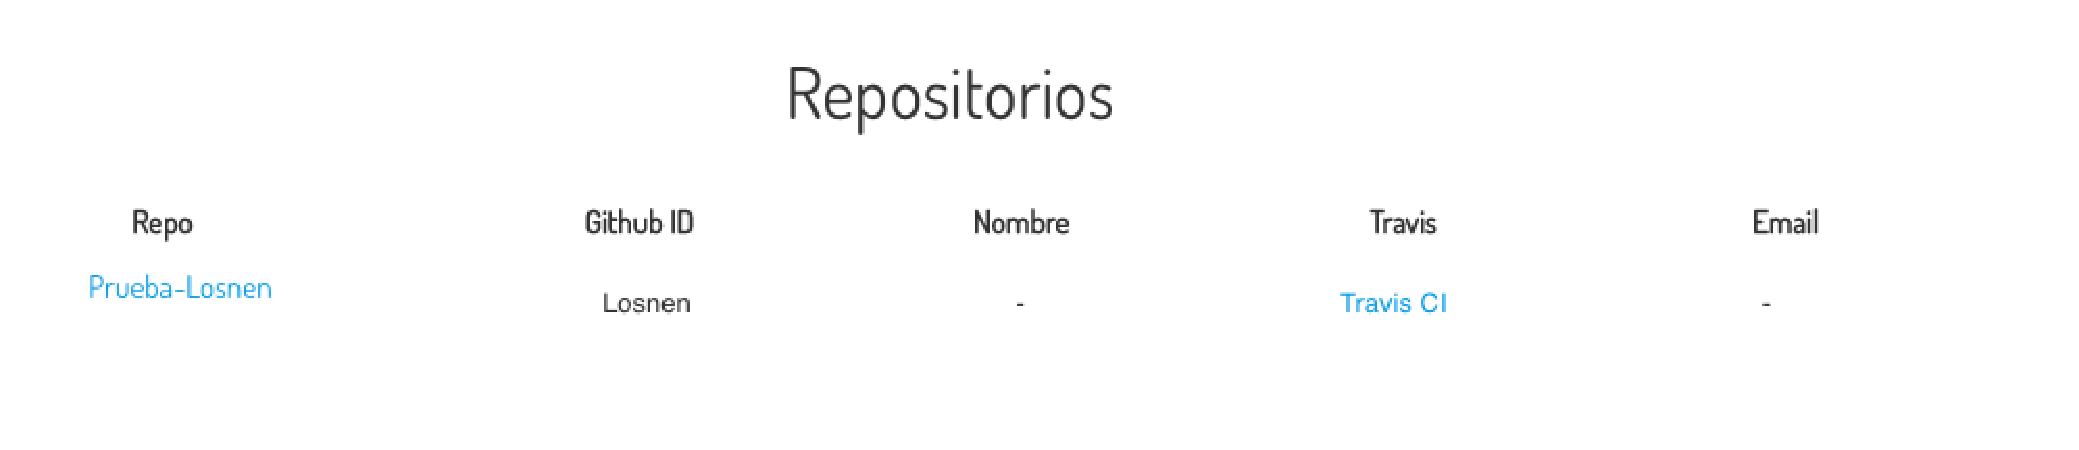
\includegraphics[scale=0.5]{images/gestion}
\caption{Gestión de tareas}
\label{fig:Gestion de tareas}
\end{center}
\end{figure}

\newpage

\subsubsection{Añadir un fichero de alumnos asociado al aula}

El mayor problema que tiene asocidar Github con la automatizacion de tareas es asociarle información a cada alumno, ya que pueden crearse una cuenta en Github con el nombre, foto o ID de github que les apetezca 
por lo que identificar a un alumno puede ser complicado. 

Por este motivo, la plataforma tiene un apartado para subir un fichero xslx o csv con información asociada a los alumnos de un aula en concreto, la información que debe ser asociada es la siguiente:

\begin{itemize}
  \item Nombre.
  \item Apellido.
  \item Dirección de correo.
  \item ID de Github.
  \item Nombre de la organización de Github que será usada como aula.
\end{itemize}

La ventaja es que el campus virtual genera un archivo en formato xslx con la mayoria de datos necesarios, salvo el ID de github de cada alumno y el nombre de la organización, es decir, el profesor tendría que solicitar al alumno su ID de github y añadir la organización de github que se usará como aula.
Por tanto, el profesor no debe escribir un fichero xslx desde cero.

\subsubsection{Crear un repositorio de evaluación de cada tarea}

Otro gran problema de automatizar la creacion de tareas es la corrección de las mismas. Desde el punto de vista de cada profesor se vuelve engorroso clonar cada repositorio, y ejecutar todos los comandos para que la práctica del alumno esté lista para corregir.

Pongamos de ejemplo la asignatura de Procesadores de Lenguajes que tiene 31 alumnos, es decir, cada tarea podría tener hasta 31 repositorios, que debería clonar uno a uno y ejecutar dentro de cada repositorio local los comandos para que funcione cada proyecto, por ejemplo npm install, para instalar las dependencias NodeJS.

La solución a este problema se propone haciendo uso del comando git combinado con la opción submodule. Git submodule nos proporciona un repositorio incrustado dentro de otro, es decir, en nuestro caso, sería un repositorio de alumno incrustado dentro de un repositorio de evaluación que contiene todos los repositorios de esa tarea, esto lo consigue medianle la creación del fichero .gitmodules, que contiene todos los repositorios submodulos. Git submodule tiene varias opciones: 

\begin{itemize}
\item git submodule init repo: Inicializa el fichero .gitmodules con el repositorio que se le pase.
\item git submodule add repo: Nos permite añadir un repositorio como submódulo del repositorio actual, crea el fichero .gitmodules si no existe.
\item git submodule update repo: Actualiza los submodulos.
\item git submodule foreach repo: Permite ejecutar un comando en cada submódulo de forma paralela.
\item git submodule sync repo: Sincroniza los submodulos con el remoto.
\end{itemize}

Una vez explicado que es git submodule y vista su utilidad veremos como se integra con Codelab y la automatización de corrección. 

Codelab crea un repositorio de corrección en Github con el nombre eval-nombre-tarea, en un principio la idea fue crear un repositorio que contuviese como sumódulos todos los repositorios de la tarea en cuestión, pero la API de Github no permite esta funcionalidad, como segunda opción se pensó crear un fichero que contuviese directamente el fichero .gitmodules, pero no funciona si el repositorio no está clonado y como última opción se crea un repositorio que contiene un pequeño script en bash que contiene una línea con el comando git submodule add <repo> por cada repositorio de alumno, de forma que al ejecutar el comando se añaden todos los repositorios de forma masiva como submódulos.

Una vez creado el repositorio de evaluación, el profesor debe clonar dicho repositorio y ejecutar el script eval.sh, añadiendo todos los repos de alumnos como submodules de forma masiva como se explicó anteriormente. Una vez hecho esto, el profesor podrá ejecutar comodamente comandos en todos los repositorios de forma paralela usando el comando git submodule foreach repo, como por ejemplo git submodule foreach 'npm i', que instala todas las dependencias de NodeJS en cada práctica.

\newpage 

\subsection{Funcionalidades para alumnos}
\label{3:6:3}

\subsubsection{Perfil}

Como alumno el usuario puede visitar el perfil, donde econtrará información básica de Github y dos pestañas, en las que el alumno tiene un historial de las tareas que ha realizado de forma grupal e individual.

\begin{figure}[!th]
\begin{center}
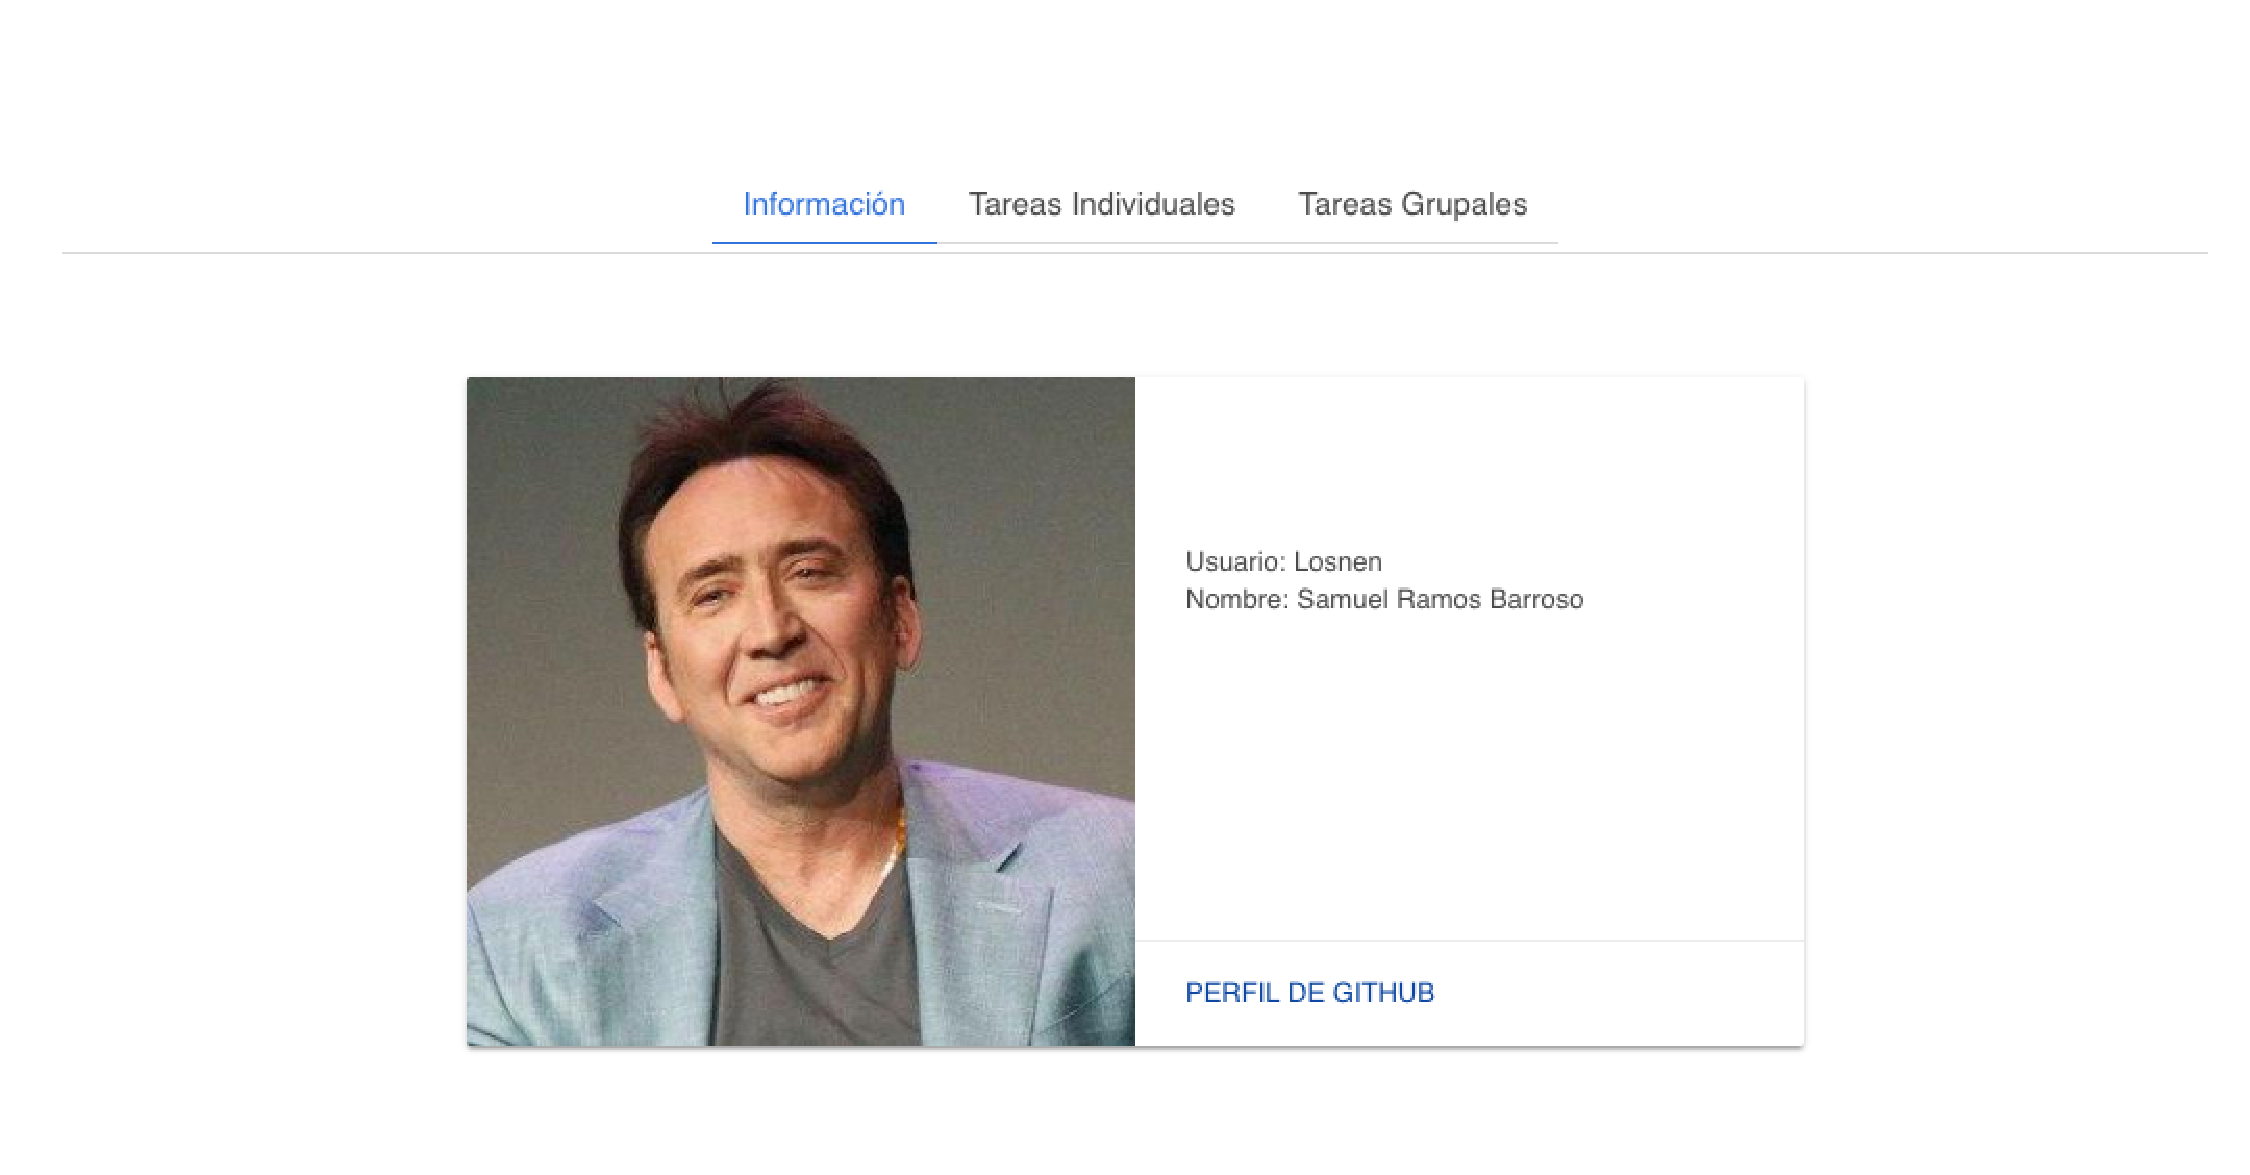
\includegraphics[scale=0.5]{images/profile}
\caption{Perfil}
\label{fig:Perfil}
\end{center}
\end{figure}

%++++++++++++++++++++++++++++++++++++++++++++++++++++++++++++++++++++++++++++++

%%%%%%%%%%%%%%%%%%%%%%%%%%%%%%%%%%%%%%%%%%%%%%%%%%%%%%%%%%%%%%%%%%%%%%%%%%%%%%%

\newpage{\pagestyle{empty}}
\thispagestyle{empty}

\chapter{Caso de uso}
\label{chapter:cuatro}

%%%%%%%%%%%%%%%%%%%%%%%%%%%%%%%%%%%%%%%%%%%%%%%%%%%%%%%%%%%%%%%%%%%%%%%%%%%%%%%
% Chapter 4: Título del capítulo 4
%%%%%%%%%%%%%%%%%%%%%%%%%%%%%%%%%%%%%%%%%%%%%%%%%%%%%%%%%%%%%%%%%%%%%%%%%%%%%%%

\section{Introducción}
\label{4:sec1}

Con vistas a probar y testear que todo funcionaba de forma correcta, Casiano me sugirió probar la plataforma para la realización de algunas prácticas individuales y grupales.
Por ello, decidimos realizar algunas tareas para la asginatura de Procesadores de Lenguajes en CodeLab.

\section{Detección de errores}
\label{4:sec2}

Al poner en uso la plataforma, los alumnos de Procesadores de Lenguajes nos ayudaron a encontrar algunos errores:

\begin{itemize}
    \item Imposibilidad de crear repositorios privados
    \item No se añadía el usuario como colaborador al repositorio.
\end{itemize}

Los alumnos utilizaron la funcionalidad de los issues para notificar el error añadiendolos en el repositorio.

Todas los errores fueron solucionados lo más rápido posible para que los alumnos de Procesadores de Lenguajes pudiesen usar la plataforma de forma correcta y realizar sus tareas en su repositorio correspondiente.
Por tanto, CodeLab se comenzó a usar en producción en un aula de 31 alumnos, demostrando que es una herramienta totalmente funcional y capaz de gestionar las tareas de código de una asignatura.

\newpage

Aparte de errores, el Casiano encontró varias mejoras que podrían ser útiles para la plataforma:

\begin{itemize}
    \item Foto y nombre del usuario en la barra de navegación.
    \item Ubicación del profesor, es decir, especificar si se encuentra en un aula o en una tarea.
    \item Elección de permisos del alumno dentro del repositorio de Github.
    \item Algunos fallos visuales como sombreados que impedían que el texto se viese de forma correcta.
\end{itemize}


Las mejoras fueron valoradas y realizadas para mejorar la interfaz gráfica y pulir ciertos defectos básicos.
Sin el test de un profesor estos defectos y mejoras hubiesen sido más complicados de encontrar y resolver.

%%%%%%%%%%%%%%%%%%%%%%%%%%%%%%%%%%%%%%%%%%%%%%%%%%%%%%%%%%%%%%%%%%%%%%%%%%%%%%%

\newpage{\pagestyle{empty}}
\thispagestyle{empty}

\chapter{Conclusiones y líneas futuras}
\label{chapter:Conclusiones}

%%%%%%%%%%%%%%%%%%%%%%%%%%%%%%%%%%%%%%%%%%%%%%%%%%%%%%%%%%%%%%%%%%%%%%%%%%%%%
% Chapter 5: Conclusiones y Trabajos Futuros 
%%%%%%%%%%%%%%%%%%%%%%%%%%%%%%%%%%%%%%%%%%%%%%%%%%%%%%%%%%%%%%%%%%%%%%%%%%%%%%%

%++++++++++++++++++++++++++++++++++++++++++++++++++++++++++++++++++++++++++++++

CodeLab nace como una herramienta que pretende extender las funcionalidades
de otras herramientas como Github Classroom, incorporando respuestas a las necesidades 
específicas del profesorado para apoyar la gestión de los cursos y
también la corrección de prácticas.

El uso de la plataforma se ha diseñado pensando en su facilidad de
uso para aquellos que no estén tan familiarizados con los conceptos
de GitHub. 

Por otro lado, se ha tenido especial cuidado en cumplir lo máximo
posible con los estándares del Software Libre,
facilitando el desarrollo colaborativo y facilitando 
la extensión de nuevas funcionalidades por parte de otros programadores.

Creemos que las facilidades que proporciona CodeLab son
útiles para aquellos profesores que tengan grupo grandes de
alumnos incluso si no están familiarizados con el entorno de Github.
CodeLab automatiza la creación de repositorios y el manejo
de los permisos de acceso de cada alumno a sus repositorios y a los
repositorios de los compañeros

Además, el control de versiones ofrece muchas ventajas a los
desarrolladores. En la actualidad, todas las empresas de desarrollo
usan control de versiones git, por lo que, es fundamental que los
alumnos aprendan a manejar git de forma correcta y aprendan técnicas
de trabajo en equipo así como todas las herramientas que proporciona
Github como los issues o los projects.

En el futuro, me planteo seguir desarrollando CodeLab, mejorándo la herramienta
y añadiendole nuevas funcionalidades. 
Una de las primeras mejoras
que se plantean es la utilización de una librería de front-end como
Vue o React para mejorar la calidad visual de la plataforma web.
Otra nueva funcionalidad que me gustaría añadir es la posibilidad
de más de un profesor por aula.


%%%%%%%%%%%%%%%%%%%%%%%%%%%%%%%%%%%%%%%%%%%%%%%%%%%%%%%%%%%%%%%%%%%%%%%%%%%%%%%
\newpage{\pagestyle{empty}}
\thispagestyle{empty}

\chapter{Summary and Conclusions}
\label{chapter:ingles}

%%%%%%%%%%%%%%%%%%%%%%%%%%%%%%%%%%%%%%%%%%%%%%%%%%%%%%%%%%%%%%%%%%%%%%%%%%%%%
% Chapter 6: Summary and Conlusions
%%%%%%%%%%%%%%%%%%%%%%%%%%%%%%%%%%%%%%%%%%%%%%%%%%%%%%%%%%%%%%%%%%%%%%%%%%%%%%%

%++++++++++++++++++++++++++++++++++++++++++++++++++++++++++++++++++++++++++++++

This chapter is compulsory.
The memory should include an extended summary and conclusions in english. 




%%%%%%%%%%%%%%%%%%%%%%%%%%%%%%%%%%%%%%%%%%%%%%%%%%%%%%%%%%%%%%%%%%%%%%%%%%%%%%%
\newpage{\pagestyle{empty}}
\thispagestyle{empty}

\chapter{Presupuesto}
\label{chapter:Presupuesto}

%%%%%%%%%%%%%%%%%%%%%%%%%%%%%%%%%%%%%%%%%%%%%%%%%%%%%%%%%%%%%%%%%%%%%%%%%%%%%
% Chapter 7: Presupuesto
%%%%%%%%%%%%%%%%%%%%%%%%%%%%%%%%%%%%%%%%%%%%%%%%%%%%%%%%%%%%%%%%%%%%%%%%%%%%%%%

%++++++++++++++++++++++++++++++++++++++++++++++++++++++++++++++++++++++++++++++

En este apartado se describirá el presupuesto del proyecto.

%---------------------------------------------------------------------------------
\section{Coste de servicios}
\label{7:sec:1}

Para el despliegue de la aplicación se han utilizado dos servidores, un servidor en Heroku que se ha usado de forma gratuita, pero que si se pagase hubiesen sido aproximadamente 30 euros en estos 4 meses que ha durado el desarrollo.

Por otro lado, el STIC ULL nos cedió una servidor virtualizado en OVirt con sistema operativo Ubuntu y una dirección IP pública para el despliegue de la aplicación web, si hubiésemos acudido a una empresa como Digital Ocean, que nos proporcionase un servidor de las mismas características nos hubiese salido 70 euros en total.

\section{Coste humano}
\label{7:sec:2}

El proyecto ha tenido una duración de 4 meses, si fuese remunerado implicaría un coste de 1.500 euros por mes según el convenio, es decir, un total de 6.400 euros por el proyecto.

\section{Coste total}
\label{7:sec:3}

El presupuesto total para realizar un proyecto de estas características sería de un total de 6.500 euros, teniendo en cuenta el coste humano y el coste de servicios.

%%%%%%%%%%%%%%%%%%%%%%%%%%%%%%%%%%%%%%%%%%%%%%%%%%%%%%%%%%%%%%%%%%%%%%%%%%%%%%%

%%%%%%%%%%%%%%%%%%%%%%%%%%%%%%%%%%%%%%%%%%%%%%%%%%%%%%%%%%%%%%%%%%%%%%%%%%%%%%%
\newpage{\pagestyle{empty}}
\thispagestyle{empty}
\begin{appendix}

\chapter{Repositorios}
\label{appendix:1}
\section{Algoritmo XXX}
\label{Apendice1:XXX}

\begin{center}
\begin{footnotesize}
\begin{verbatim}

***********************************************************************************
*
* Fichero .h
*
***********************************************************************************
*
* AUTORES
*   
*
* FECHA
*   
*
* DESCRIPCION
*   
*
************************************************************************************/

\end{verbatim}
\end{footnotesize}
\end{center}

\section{Algoritmo YYY}
\label{Apendice1:YYY}

\begin{center}
\begin{footnotesize}
\begin{verbatim}


/***********************************************************************************
 *
 * Fichero .h
 *
 ***********************************************************************************
 *
 * AUTORES
 *
 * FECHA
 *
 * DESCRIPCION
 *
 *
 ************************************************************************************/

\end{verbatim}
\end{footnotesize}
\end{center}


\end{appendix}

%%%%%%%%%%%%%%%%%%%%%%%%%%%%%%%%%%%%%%%%%%%%%%%%%%%%%%%%%%%%%%%%%%%%%%%%%%%%%%%
\addcontentsline{toc}{chapter}{Bibliografía}
\bibliographystyle{plain}

\bibliography{memtfg}
\nocite{*}

%%%%%%%%%%%%%%%%%%%%%%%%%%%%%%%%%%%%%%%%%%%%%%%%%%%%%%%%%%%%%%%%%%%%%%%%%%%%%%%

\end{document}
